\section{Results}
\subsection{Network Statistics CHANGE}
SEEM was found to be the set of networks closest to the CENN in average edge distance (see table 1 and fig 1). [INSERT STATS FOR STATISTICAL SIGNIFICANCE BETWEEN DISTRIBUTIONS]. RDDAM were closest to the CENN in average clustering coefficient and number of bidirectional links. [INSERT STATS FOR STATISTICAL SIGNIFICANCE BETWEEN DISTRIBUTIONS]. These results were not heavily dependent on which network was chosen.

\begin{table}[h]
  \import{}{../data/spreadsheets/data}
  \caption{INSERT HERE}
\end{table}

\begin{figure}[h]
  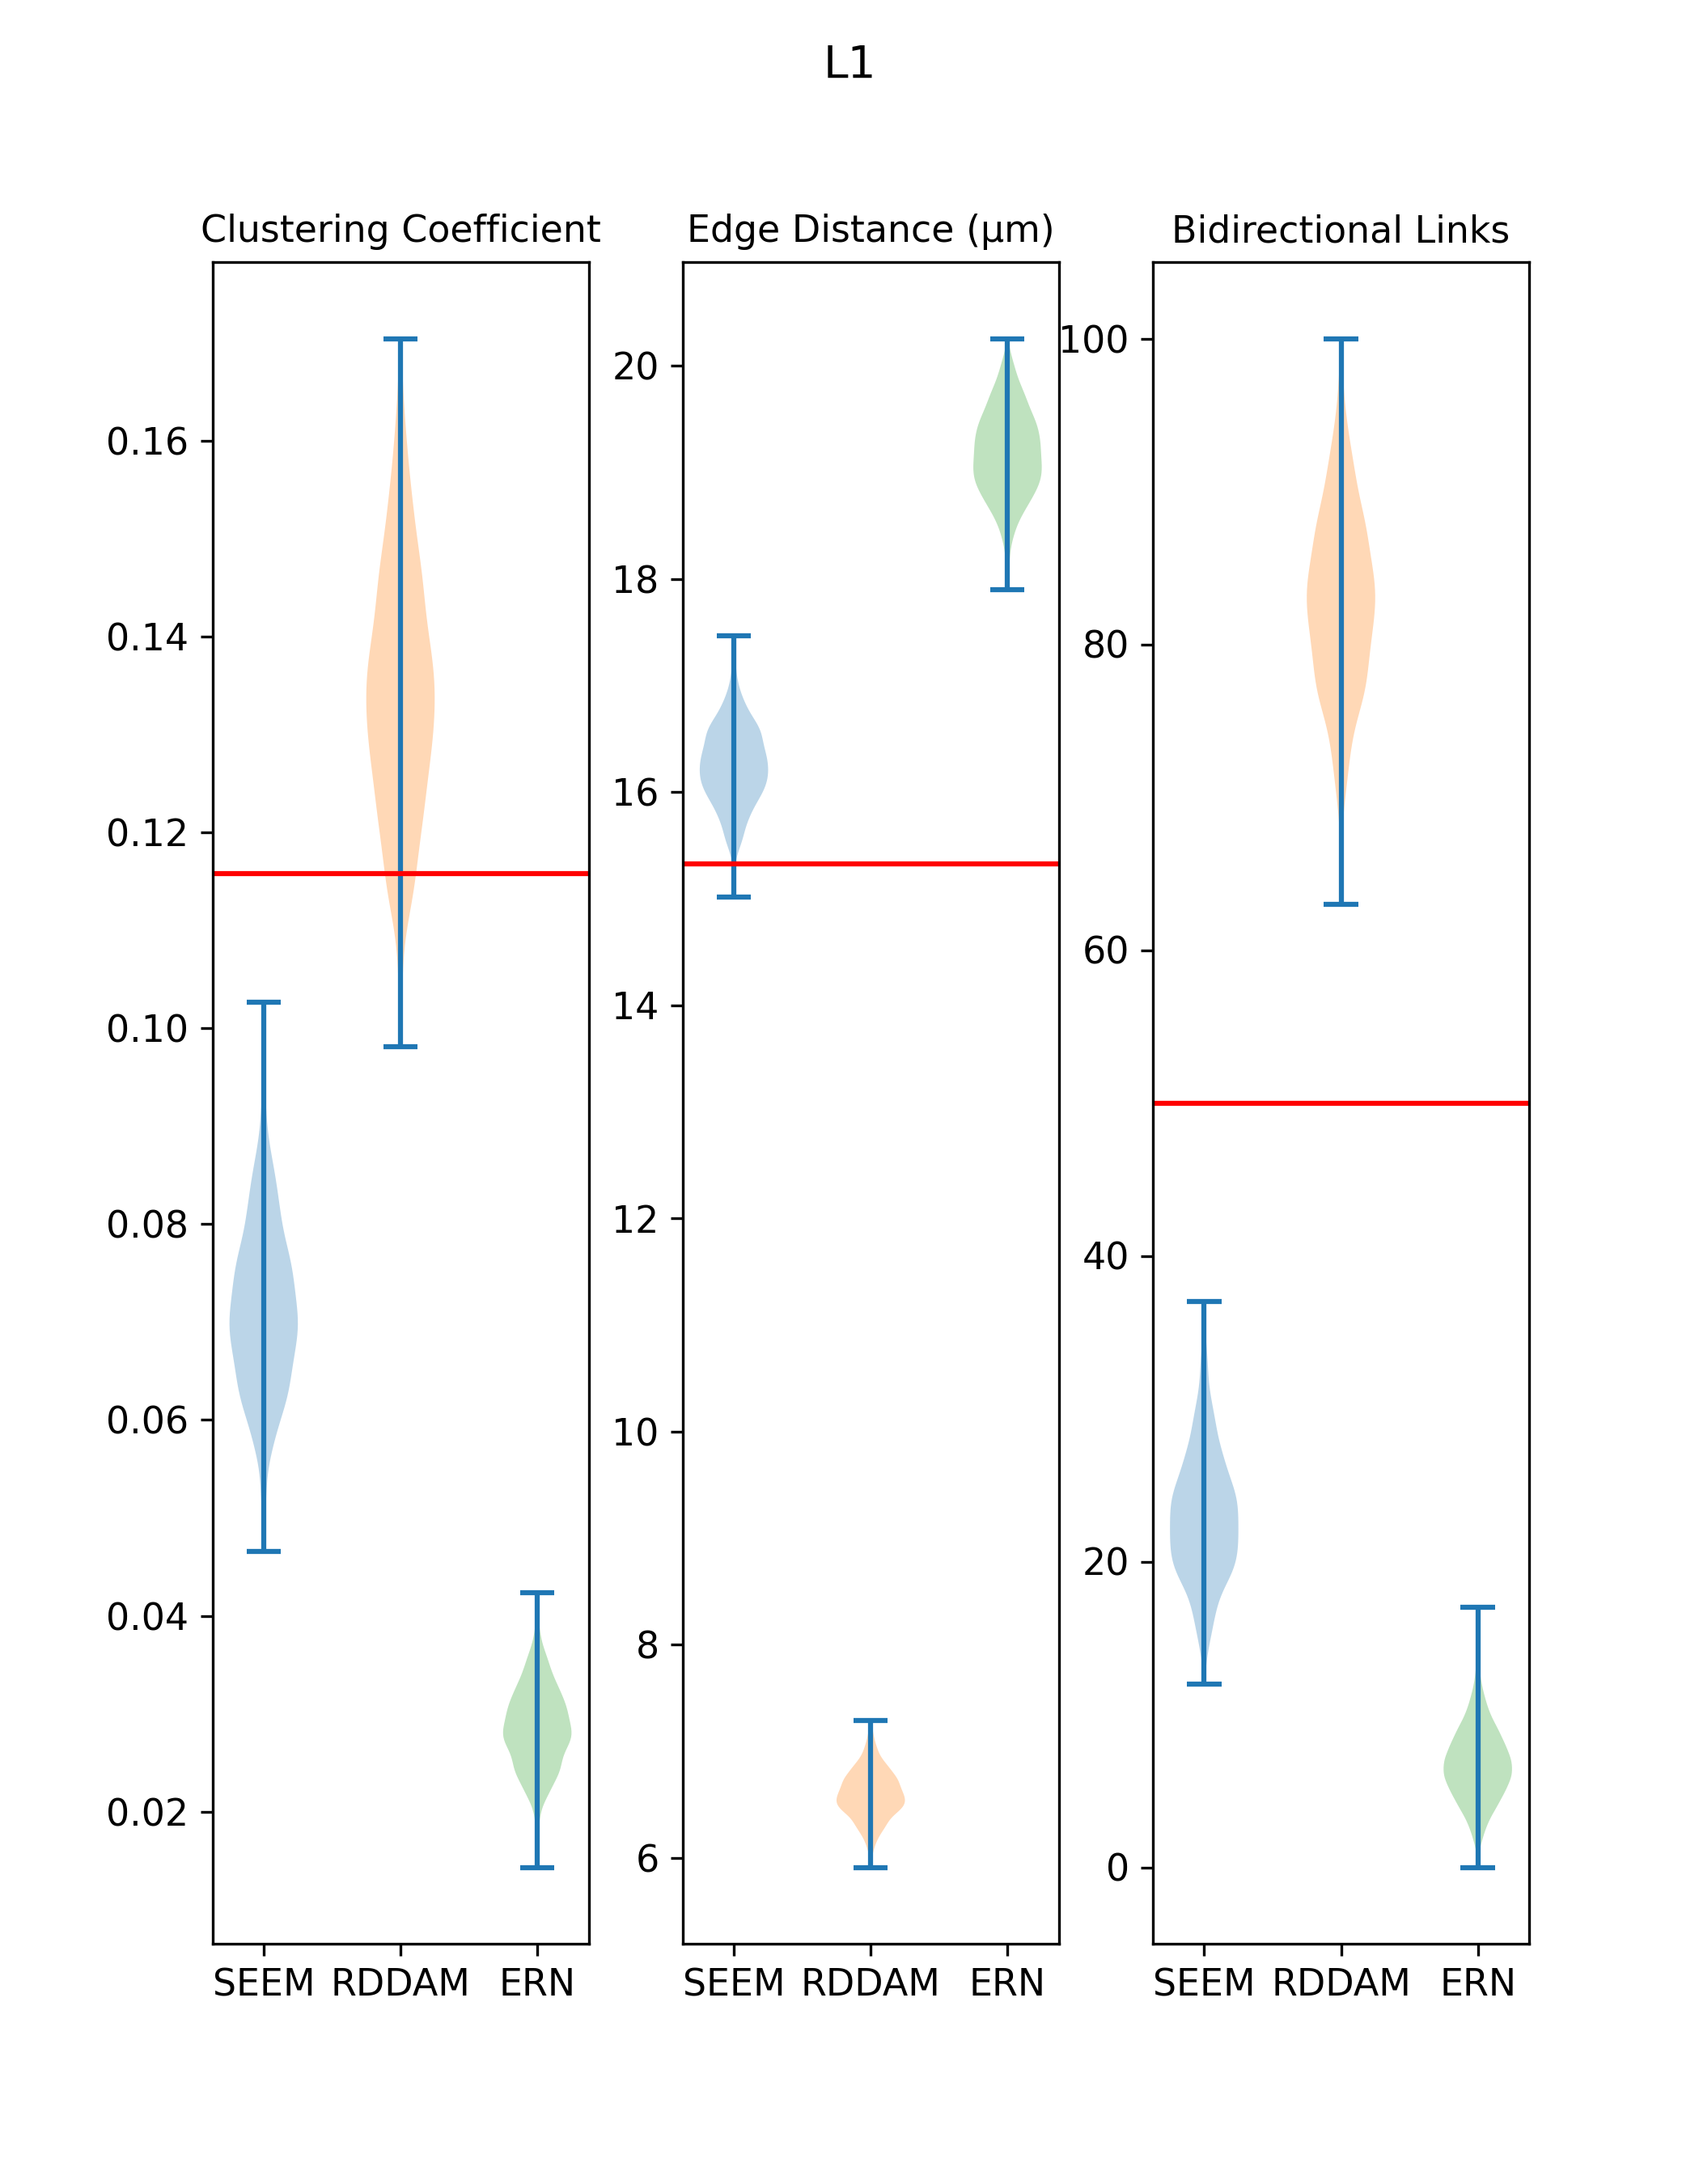
\includegraphics[width=\linewidth]{../data/images/stats/L1.png}
  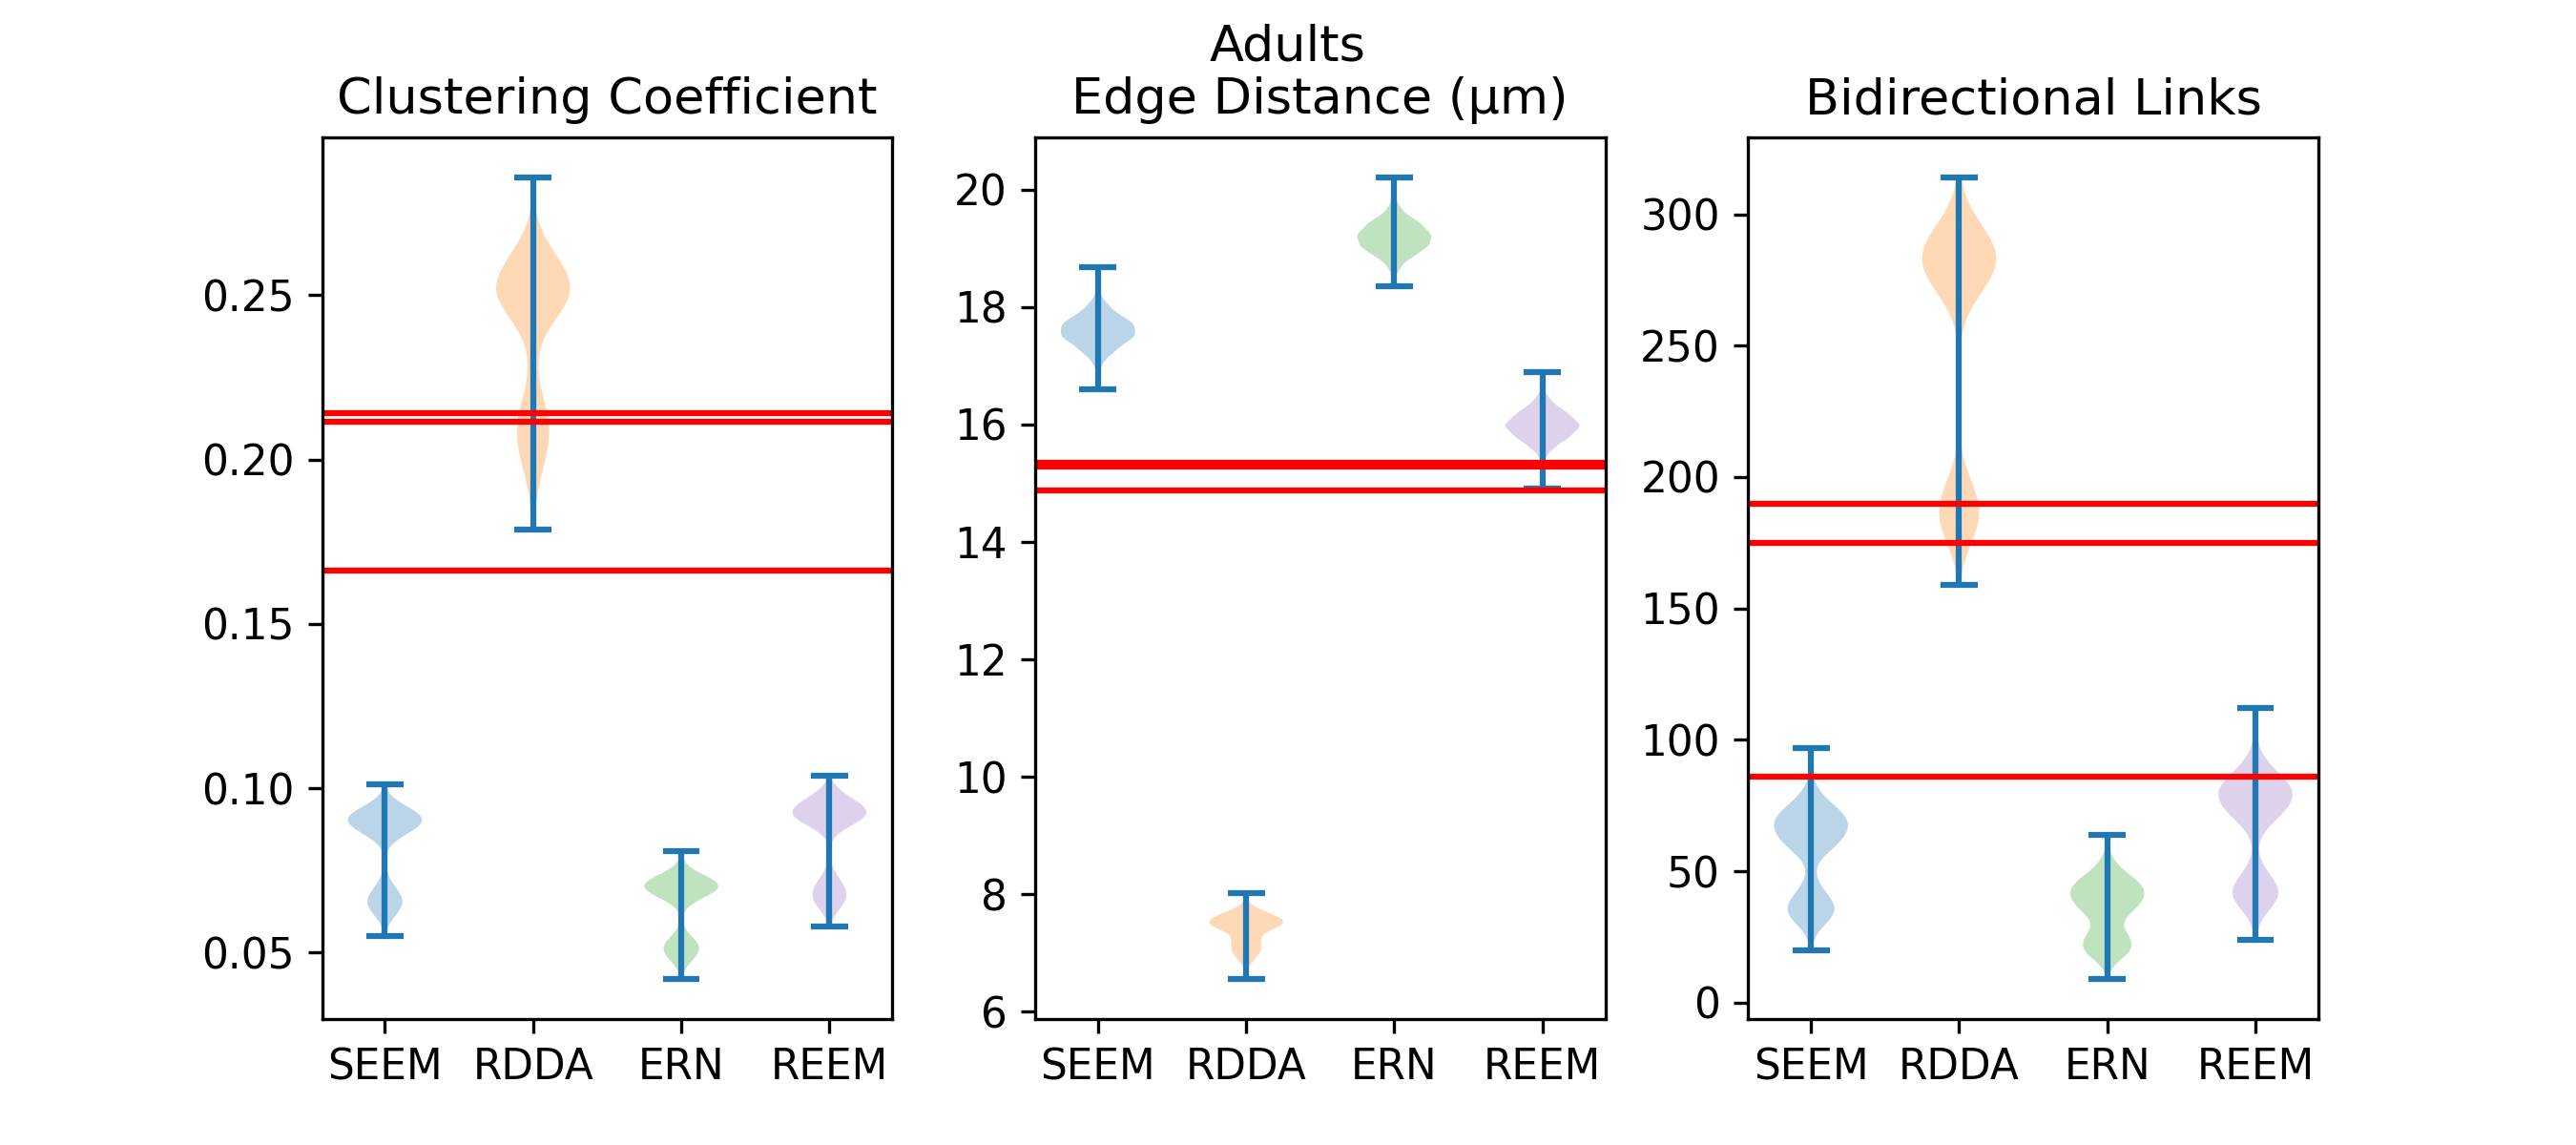
\includegraphics[width=\linewidth]{../data/images/stats/Adults.png}
  \caption{INSERT HERE}
\end{figure}

The degree distributions of RDDAM were also found to be most similar to the CENN with a Wasserstein Distance of 0.005 in L1 and 0.002 in adults (see fig 2). SEEM was close with a Wasserstein Distance of 0.006 in L1 and 0.003 in adults, making the distinction between the two insignificant. The degree distributions of Erdos-Renyi graphs appeared much less like the CENN with a Wasserstein Distance of 0.013 in L1 and 0.009 in adults. The average degree between all four graphs were not significantly different.

\begin{figure}[h]
    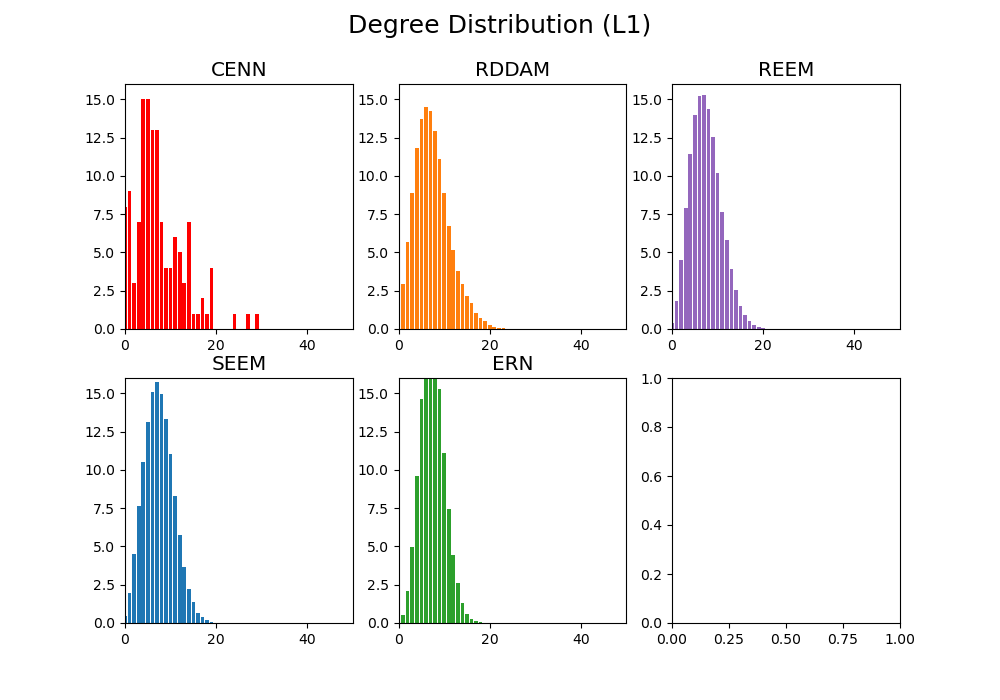
\includegraphics[width=0.75\linewidth]{data/images/distributions/degreeDist_W1_Rand.png}
    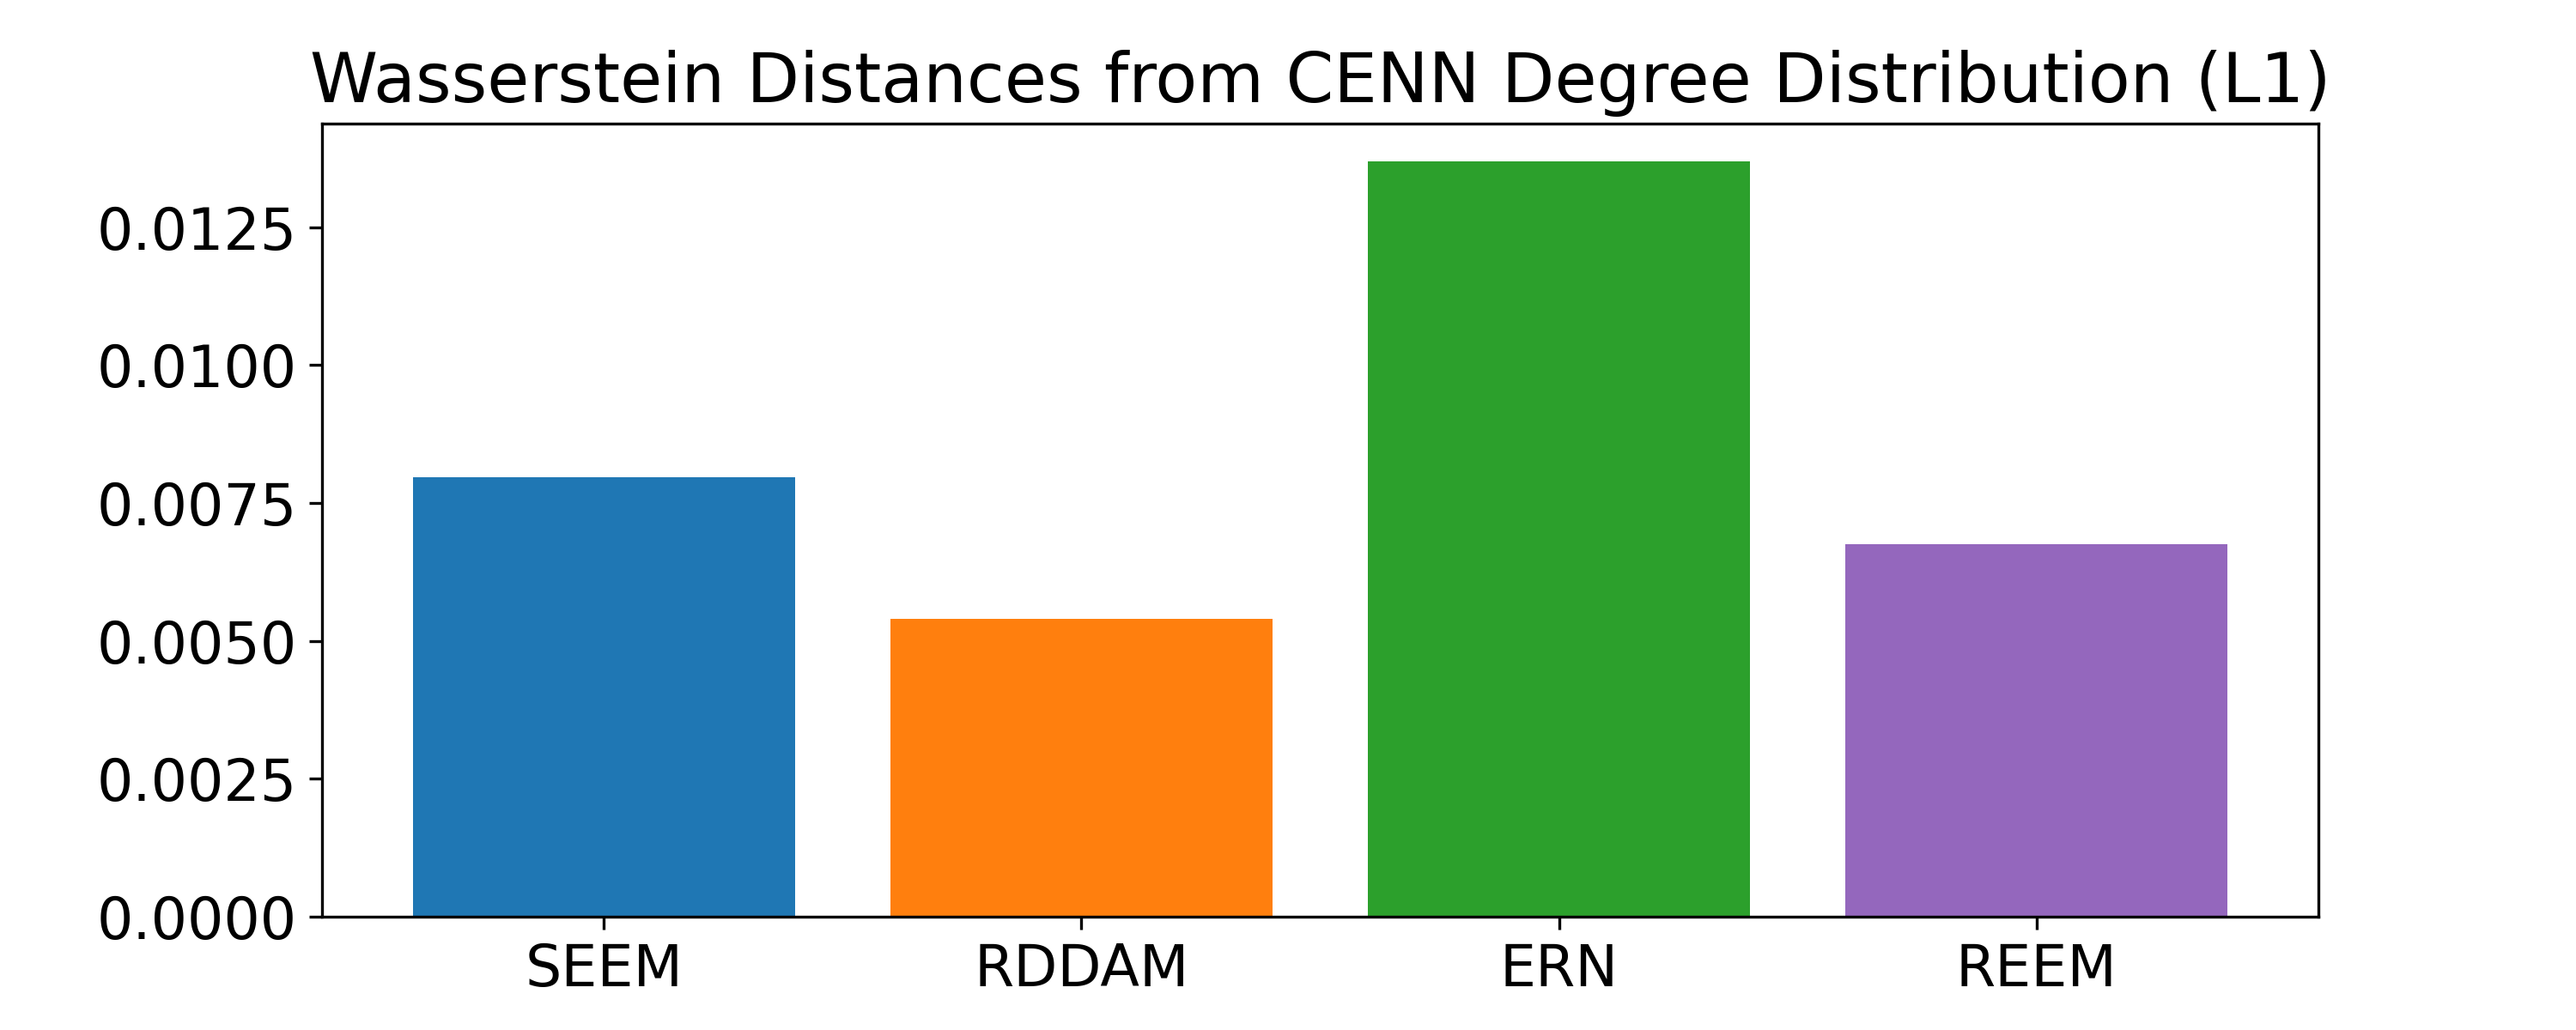
\includegraphics[width=0.24\linewidth]{data/images/compareDistributions/wassersteinDistances_Degree_L1_2.png}

    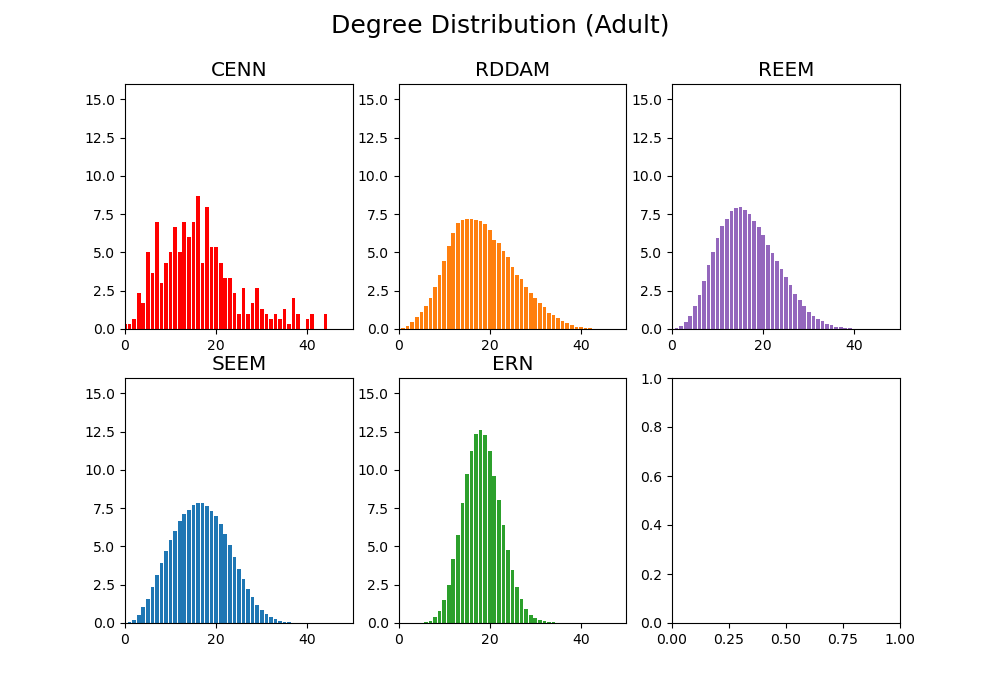
\includegraphics[width=0.75\linewidth]{data/images/distributions/degreeDist_L5_Rand.png}
    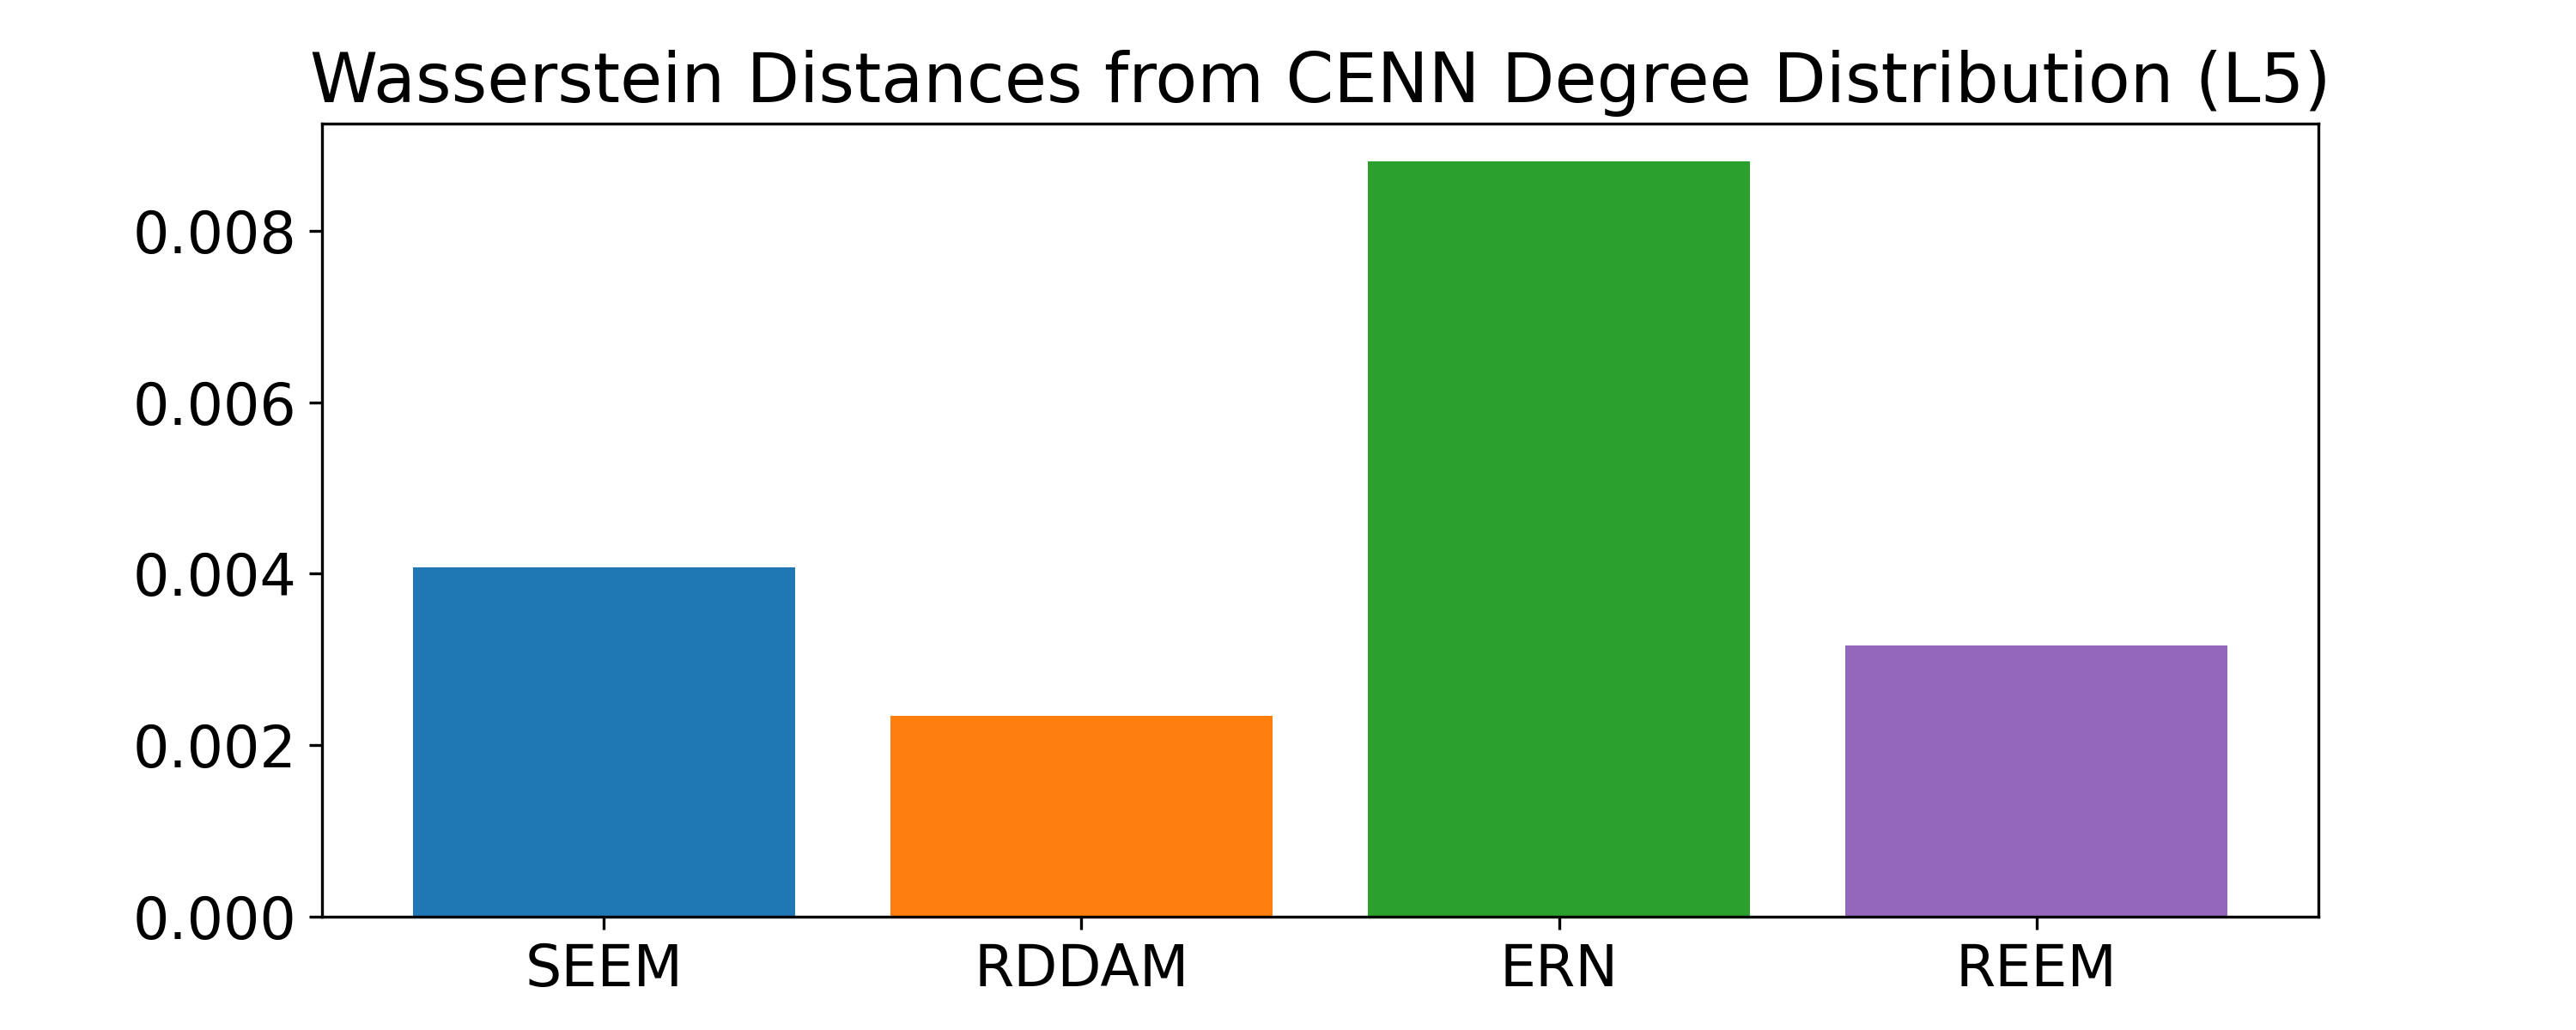
\includegraphics[width=0.24\linewidth]{data/images/compareDistributions/wassersteinDistances_Degree_L5_2.png}
  \caption{INSERT HERE}
\end{figure}

Comparing the distribution of edge distances shows a different picture. Here, the resulting graphsof SEEM were found to be closest to the CENN (see fig 3). The edge distance distributions in SEEM had a Wasserstein Distance of 0.004 in L1 and 0.003 in adults. The Erdos-Renyi graphs, with a Wasserstein Distance of 0.005 in L1 and 0.004 in adults, were even more similar to CENN than the RDDAM, with a Wasserstein Distance of 0.013 in L1 and adults. These results distinguish SEEM from RDDAM, showing the proclivity of RDDAM to form very short connections, something SEEM does not appear to do.

\begin{figure}[h]
    \includegraphics[width=0.75\linewidth]{data/images/distributions/distDist_W1_Rand.png}
    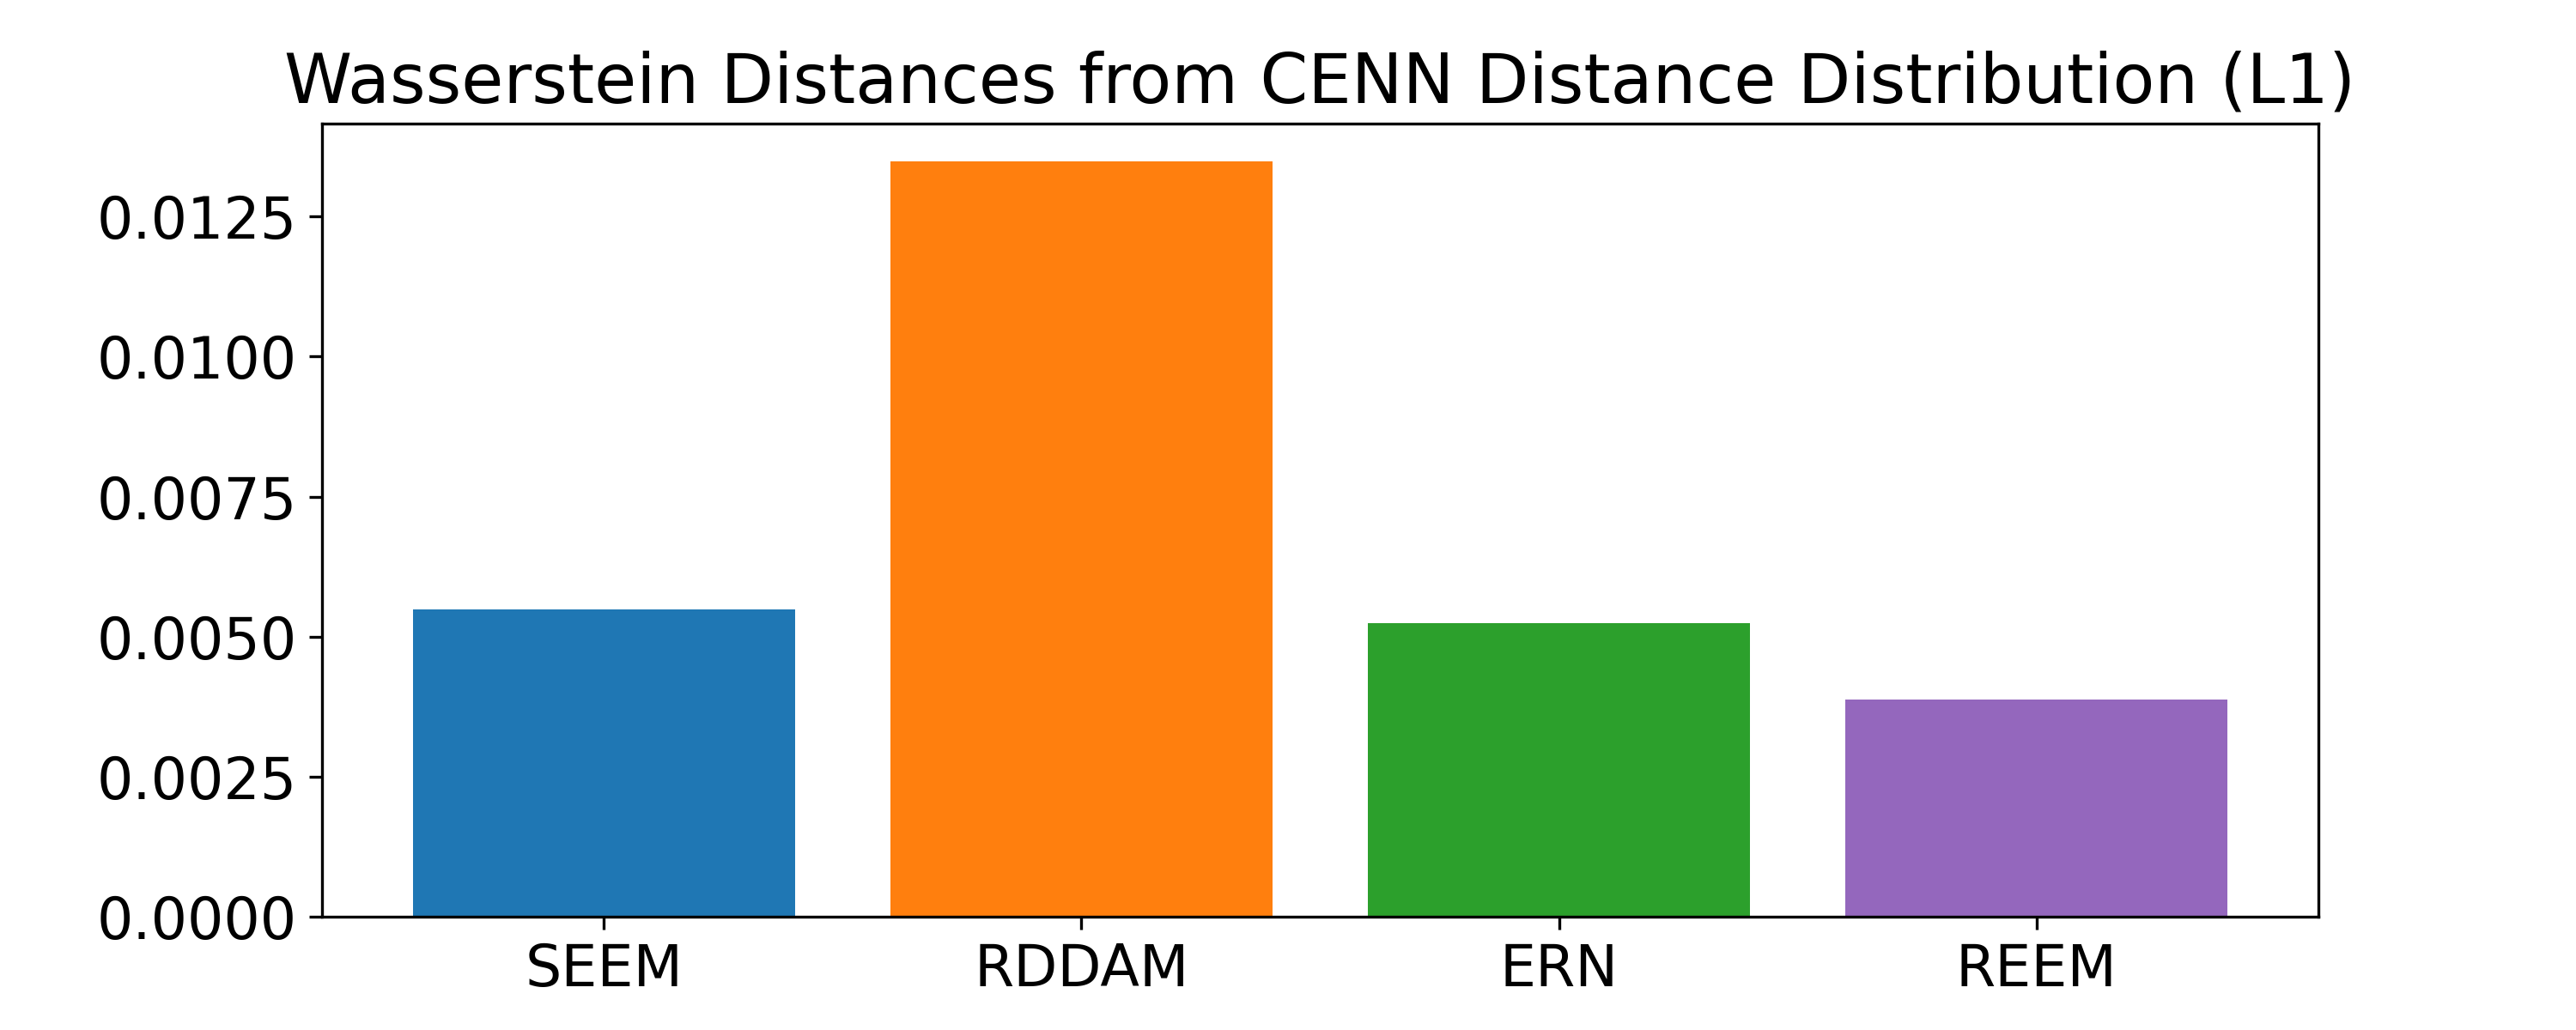
\includegraphics[width=0.24\linewidth]{data/images/compareDistributions/wassersteinDistances_Distance_L1_2.png}

    \includegraphics[width=0.75\linewidth]{data/images/distributions/distDist_L5_Rand.png}
    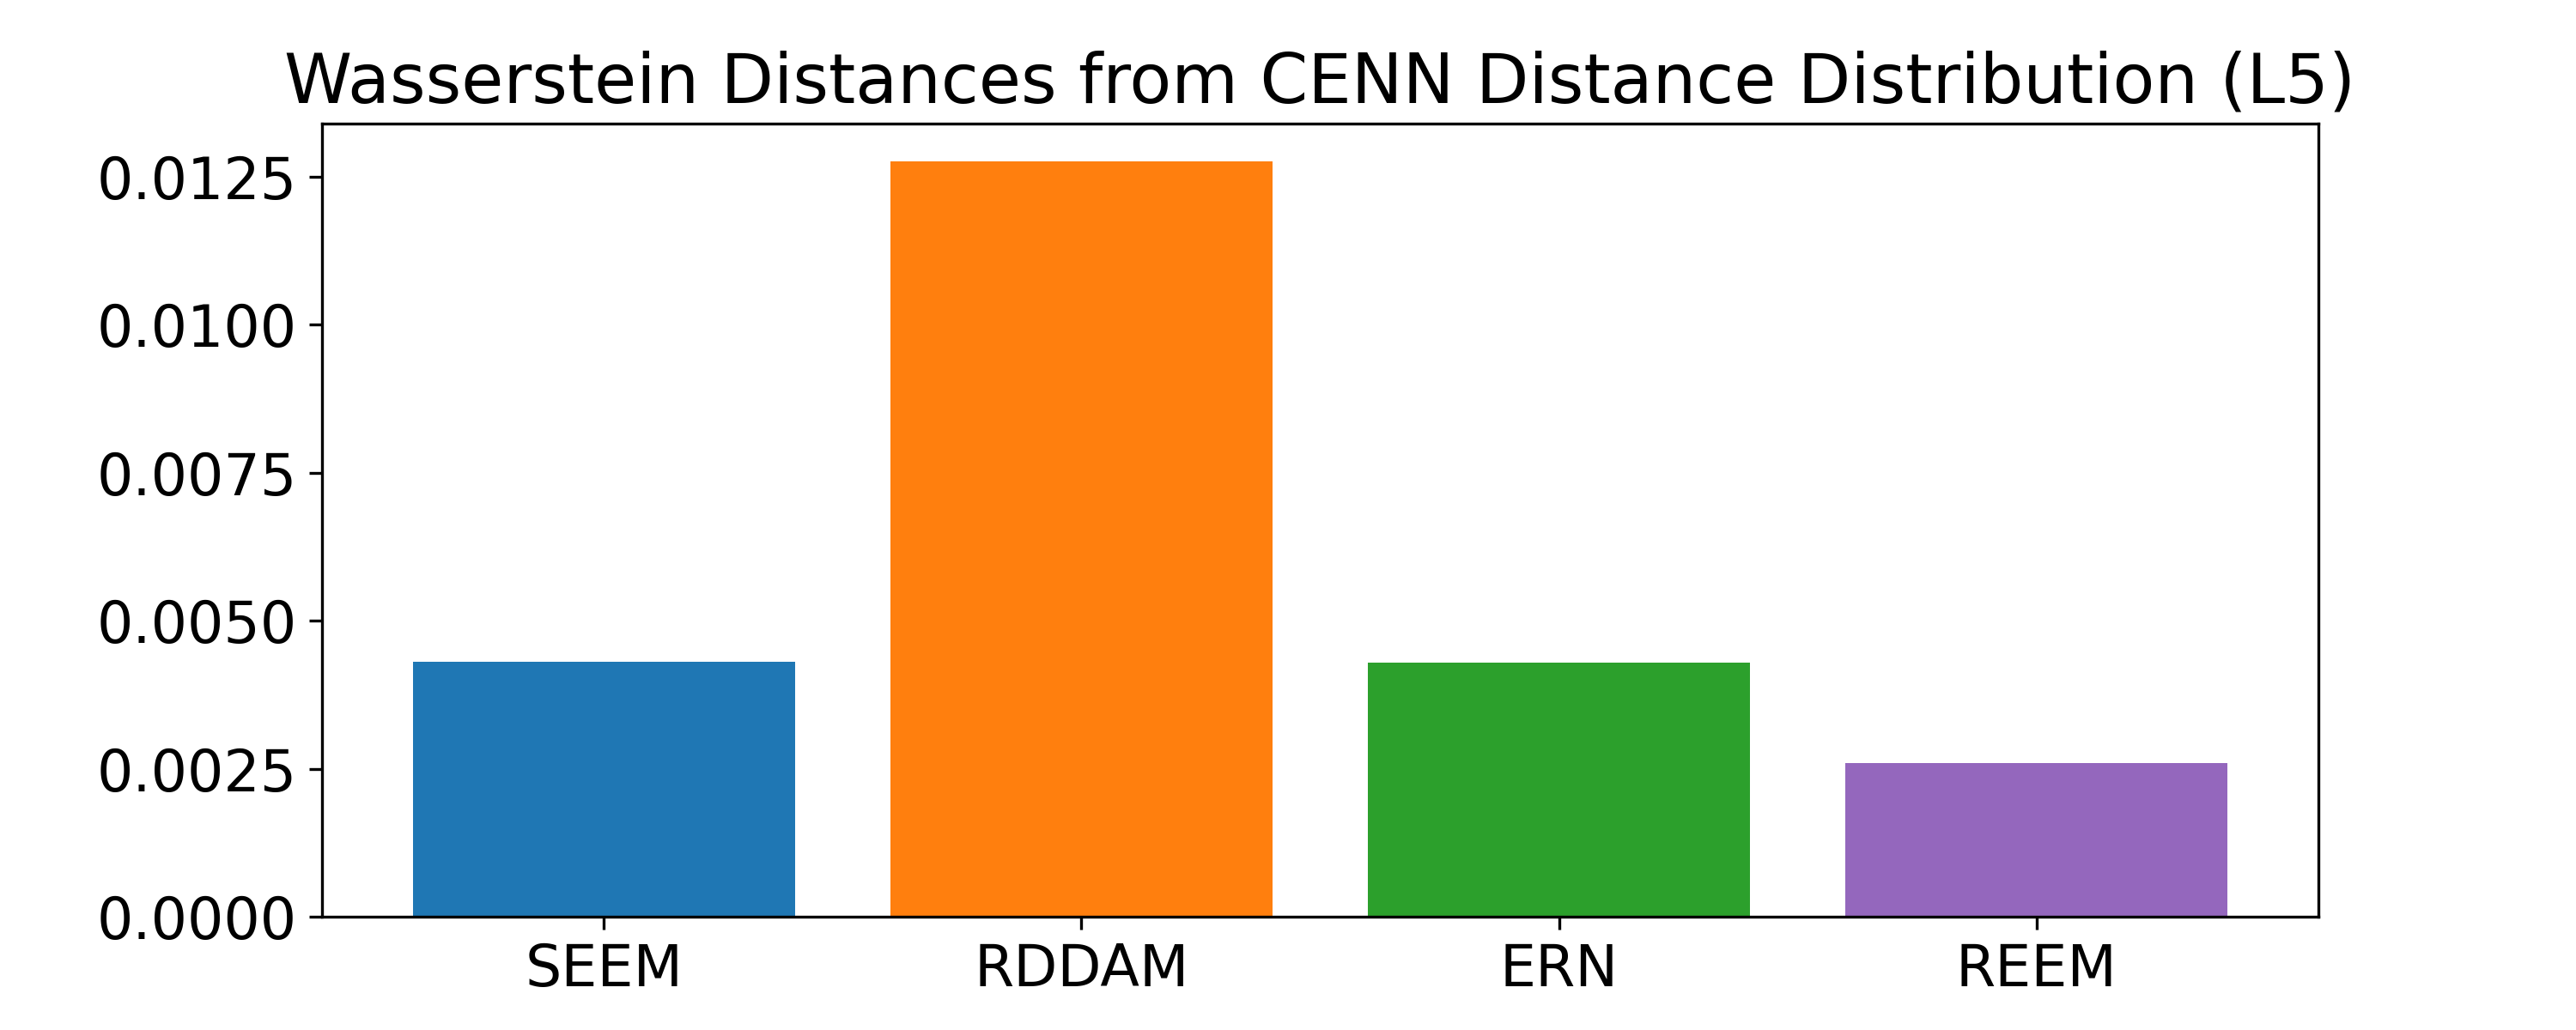
\includegraphics[width=0.24\linewidth]{data/images/compareDistributions/wassersteinDistances_Distance_L5_2.png}
  \caption{INSERT HERE}
\end{figure}

Spatially embedding these graphs using provided coordinates resulted in a particular connectivity pattern shared between the CENN and SEEM graphs (see Figure 4). [INSERT DATA ABOUT DISTRIBUTION OF CROSS-PHARYNX CONNECTIONS]